\documentclass[11pt,letterpaper]{article}
\usepackage[T1]{fontenc}
\usepackage{fullpage}
\usepackage[top=2cm, bottom=4.5cm, left=2.5cm, right=2.5cm]{geometry}
\usepackage{amsmath,amsfonts,amssymb}
\usepackage{lastpage}
\usepackage[inline]{enumitem}
\usepackage{fancyhdr}
\usepackage{mathrsfs}
\usepackage{xcolor}
\usepackage{graphicx}
\usepackage{subcaption}
\usepackage{appendix}
\usepackage{hyperref}
\usepackage{titlesec}
\usepackage{fancyvrb}
\hypersetup{colorlinks=true, linkcolor=blue, linkbordercolor={0 0 1}}

%\renewcommand{\arraystretch}{1.5}
\titlespacing*{\section}{0pt}{0.65\baselineskip}{0.5\baselineskip}

\setlength{\parindent}{0.0in}
\setlength{\parskip}{0.05in}

\newcommand{\qrf}{\texttt{QRFactor}}

\pagestyle{fancyplain}
\lhead{}
\chead{GPU Solutions for PSCAD: IT17112}
\rhead{}
\cfoot{\small\thepage}
\headsep 32pt

%%%%%%%%%%%%%%%%%%%%%%%%%%%%%%%%%%%%%%%%%%%%%%%%%%%%%%%%%%%%%%%%%%%%%%%%%%%%%%%
%%%%%%%%%%%%%%%%%%%%%%%%%%%%%%%%%%%%%%%%%%%%%%%%%%%%%%%%%%%%%%%%%%%%%%%%%%%%%%%

\begin{document}
\begin{center}
    {\Large \bf Monthly Summary: December, 2020 \& January, 2021}
\end{center}

During this period, the full functionality -- both device-side and host-side functions -- of \qrf~was incorporated into a DLL (Dynamic Link Library) version and documentation was created to reflect these changes. To produce a DLL that is compiler independent, wrapper functions were created that take and return QRFactor-type pointers. In \S\!~\ref{sec: client}, we show how the QRFactor DLL is used by a client program.

The inclusion of GPU functions meant that the DLL template available in Visual Studio was not immediately applicable. Instead, customization of the template was required. See \S\!~\ref{sec: gpu dll} for details.

Following a December meeting with the UW and MHI teams, additional changes to QRFactor were discussed that would allow for better integration will future PSCAD EMT updates. These additional changes are outlined in \S\!~\ref{sec: additions} and are currently being implemented.

\section{Using QRFactor DLL Within a Client Program}
\label{sec: client}

As mentioned above, the QRFactor DLL was written to be compiler-independent and does this by taking and returning typed pointers, which are then converted into void types upon compilation. With this structure in mind, a client program uses the QRFactor DLL in the following way:
\begin{verbatim}
    #include "qrgpu.h"  // Header file for QRFactor library

    int main()
    {
        double* inPtr;  // Pointer to column-major dense matrix  
        int* rPtr;      // Pointer to number of rows
        int* cPtr;      // Pointer to number of columns
        int* nnz;       // Pointer to total number of non-zero values

        /*
        * Create an instance of QRFactor with the total number of
        * non-zero values as an input
        */
        QRFactor* qr = QR_Create(*nnz);

        /*
        * Build the non-zero entries with the input matrix. Repeat as
        * many times as required until all subsystems have been read in
        */ 
        qr = QR_buildTriplets(qr, inPtr, *rPtr, *cPtr);
        
        /*
        * Assuming all subsystems have been read in, now build the
        * full system sparse matrix and convert to CSR storage
        */
        qr = QR_buildSparseMatrix(qr);

        /*
        * Use GPU-based factoring method on the full system matrix
        */
        qr = QR_factor(qr);
    
        /* 
        * The matrix has been factored and is held on the GPU. Solve 
        * the linear system for each set of input data.
        */
        double* b1;      // Pointer to input vector
        double* x1;      // Pointer to variable vector
        qr = QR_solve(qr, const_cast<double*>(b1), x1);

        double* b2;      // Pointer to input vector
        double* x2;      // Pointer to variable vector
        qr = QR_solve(qr, const_cast<double*>(b2), x2);

        /*
        * Memory cleanup
        */
        QR_delete(qr);

        return 0;
    }
\end{verbatim}


\section{Creating a DLL with Device-side Functions in Microsoft Visual Studio 2019}
\label{sec: gpu dll}
Beginning with a CUDA runtime template project in VS2019, several adjustments are required to create a DLL with CUDA functions. In particular, the project's General Properties page must be changed so that the Configuration Type is Dynamic Library (.dll). See figure~\ref{fig: gen props} for a screenshot. Other library linking, such as to the CUDA Toolkit, should be included with the CUDA runtime template

\begin{figure}[h]
    \centering
    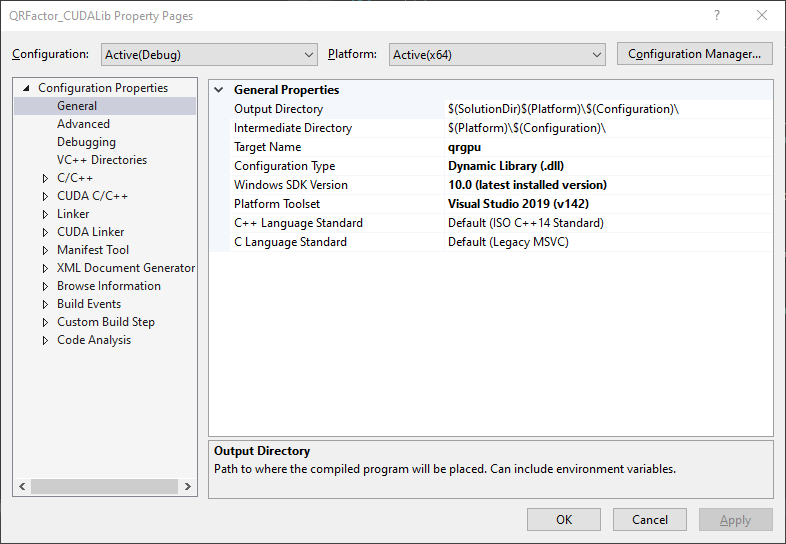
\includegraphics[width=0.75\textwidth]{DLL_GeneralProperties.png}
    \caption{A snapshot of Configuration Properties $\to$ General tab after a CUDA runtime template is changed to a DLL project.}
    \label{fig: gen props}
\end{figure}

By examining the contents of a \href{https://docs.microsoft.com/en-us/cpp/build/walkthrough-creating-and-using-a-dynamic-link-library-cpp?view=msvc-160}{C++ DLL template}, we see that there are several files provided by VS2019 that are required to build a DLL: ``framework.h,'' ``pch.h,'' ``dllmain.cpp,'' and ``pch.cpp''. These short files provide entry points for the DLL applications and must be in each new project. Therefore, they must be added to the CUDA DLL solution as well. See \S\!~\ref{sec: dll template} for these files.

The user then creates a new header file that contains the library contents. Within the header file, any function declarations that are accessible to the client program must be wrapped with import/export macros and the \verb+EXTERN+ keyword. As an example, the following code defines the import/export macro \verb+QRGPU_API+ and the \verb+EXTERN+ keyword before declaring the example function \verb+function+:

\newpage 

\begin{verbatim}
    #ifdef QRGPU_EXPORTS
    #define QRGPU_API __declspec(dllexport)
    #else
    #define QRGPU_API __declspec(dllimport)
    #endif

    #ifdef __cplusplus			
    #define EXTERN
    #else
    #define EXTERN extern "C"
    #endif

    EXTERN QRGPU_API function;      // Example function declaration
\end{verbatim}

\section{Using a Custom CUDA DLL in a Client Program in Microsoft Visual Studio 2019}

Having created the custom DLL, a VS2019 client program can use the library once it has been properly linked. After creating a new Console Project in VS2019, we add the path to the CUDA DLL as well as any libraries that the DLL may rely on (in this example, the Eigen library and CUDA Toolkit libraries are also included) in the C++ Additional Include Directories. See figure~\ref{fig: client includes}.

\begin{figure}
    \centering
    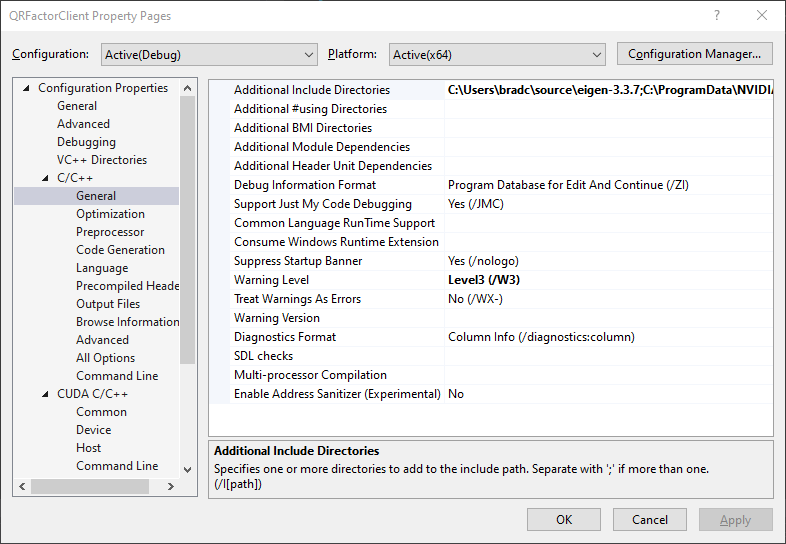
\includegraphics[width=0.6\textwidth]{DLL_ClientIncludes.png}
    \caption{A snapshot of Configuration Properties $\to$ C/C++ $\to$ General tab in a client program. The CUDA DLL directory must be included in the Additional Include Directories, as well as any libraries that it may depend on.}
    \label{fig: client includes}
\end{figure}

Next, the CUDA DLL library must be pointed to directly by specifying the path of the \verb+#include+ declaration. This is set in the Linker General options, as seen in figure~\ref{fig: linker}. Note that the \verb+$(IntDir)+ macro will allow for the linking of either a \emph{Debug} or \emph{Release} version of the DLL to be linked. Also in the Linker options, the name of the CUDA DLL itself must be added on the Input tab under Additional Dependencies, as shown in figure~\ref{fig: dependencies}.

\begin{figure}
    \centering
    \begin{subfigure}[t]{0.48\textwidth}
        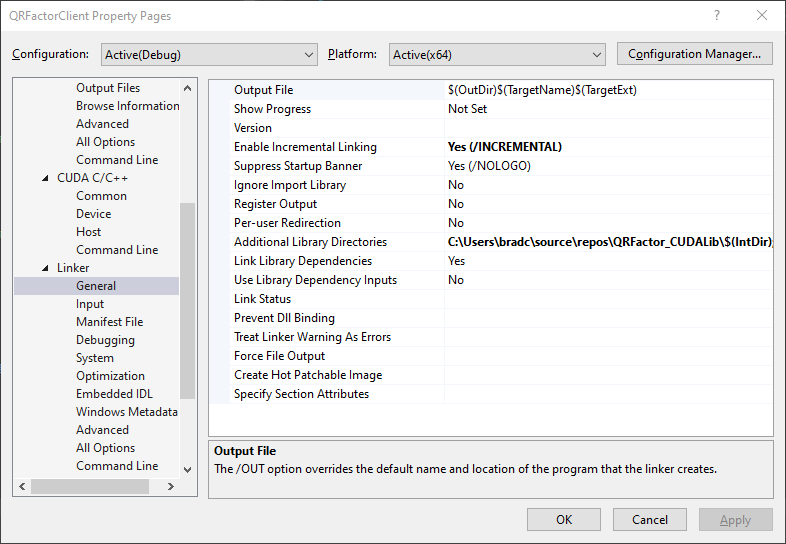
\includegraphics[width=\textwidth]{DLL_ClientLinkerGeneral.png}
        \caption{A snapshot of Linker $\to$ General tab in a client program. Under Additional Library Directories, the path to the CUDA DLL is added.}
        \label{fig: linker}
    \end{subfigure}
    \hfill
    \begin{subfigure}[t]{0.48\textwidth}
        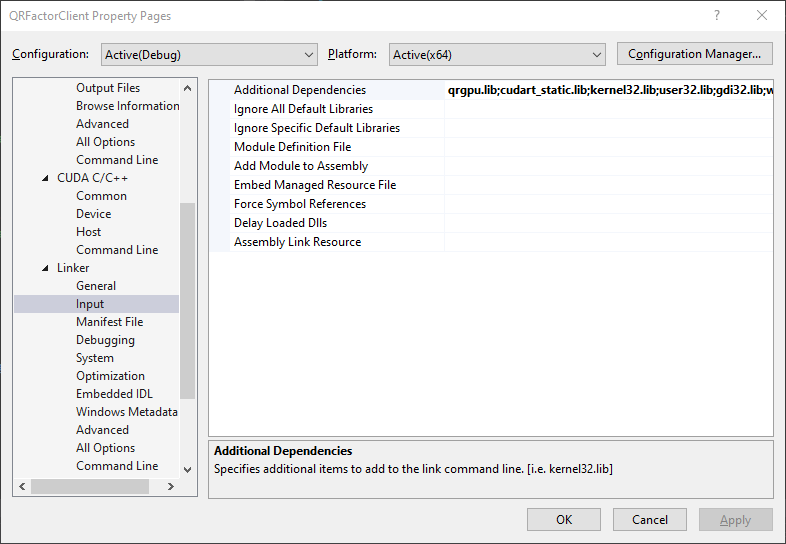
\includegraphics[width=\textwidth]{DLL_CLientLinkerInput.png}
        \caption{A snapshot of Linker $\to$ Input tab in a client program. Under Additional Dependencies, the name of the library is included.}
        \label{fig: dependencies}
    \end{subfigure}
    \caption{Linker options in the client program.}
\end{figure}

Finally, a Post-Build process must be added to copy the CUDA DLL into the client program's build output directory. This is done through the Build Events options by specifying a Post-Build Event. In the Command Line field, the CUDA DLL (named ``example.dll'') is copied directly into the build directory using
\begin{center}
\begin{verbatim}
    xcopy /y /d "Path\to\Library\$(IntDir)example.dll" "$(OutDir)"
\end{verbatim}
\end{center}
See figure~\ref{fig: post build} for a snapshot. After these options have been set, the client program invokes the CUDA DLL using the standard \verb+#include+ macro.

\begin{figure}
    \centering
    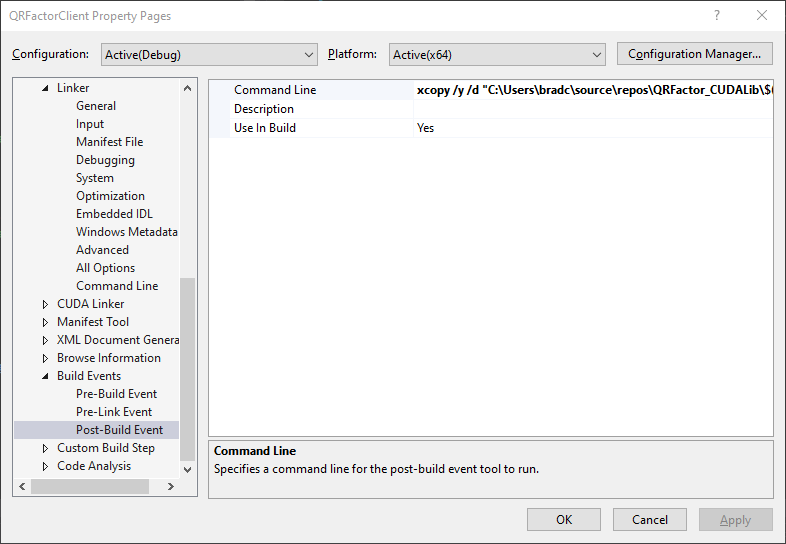
\includegraphics[width=0.6\textwidth]{DLL_ClientPostBuild.png}
    \caption{A snapshot of Build Events $\to$ Post-Build Event tab in a client program. The CUDA DLL is copied into the client program output directly as a post-build event.}
    \label{fig: post build}
\end{figure}

\section{Pending Additions}
\label{sec: additions}
The following additions to the QRFactor DLL were discussed and are currently being implemented:
\begin{itemize}
    \item Check whether a GPU is connected and return an error if the library is not able to run on the existing architecture.
    \item Use a map container to trace the positions of the submatrices within the larger full system matrix. This can be used later to quickly identify subsystems with values that change within the EMT system being studied, allowing the system matrix to be rapidly rapidly updated without requiring reassembly.
\end{itemize}

\section{DLL Template Files}
\label{sec: dll template}
These files are part of a C++ DLL template which, when constructing a CUDA DLL, must be added by hand. They are included here for reference.

%\noindent\rule{\textwidth}{1pt}

\section*{\texttt{pch.h}}
\begin{verbatim}
#ifndef PCH_H
#define PCH_H

// add headers that you want to pre-compile here
#include "framework.h"

#endif //PCH_H
\end{verbatim}
\section*{\texttt{pch.cpp}}
\begin{verbatim}
// pch.cpp: source file corresponding to the pre-compiled header
#include "pch.h"

// When you are using pre-compiled headers, 
// this source file is necessary for compilation to succeed.
\end{verbatim}
\section*{\texttt{framework.h}}
\begin{verbatim}
#pragma once

#define WIN32_LEAN_AND_MEAN   // Exclude rarely-used stuff from Windows headers
// Windows Header Files
#include <windows.h>
\end{verbatim}
\section*{\texttt{dllmain.cpp}}
\begin{verbatim}
// dllmain.cpp : Defines the entry point for the DLL application.
#include "pch.h"

BOOL APIENTRY DllMain(HMODULE hModule,
    DWORD  ul_reason_for_call,
    LPVOID lpReserved
)
{
    switch (ul_reason_for_call)
    {
    case DLL_PROCESS_ATTACH:
    case DLL_THREAD_ATTACH:
    case DLL_THREAD_DETACH:
    case DLL_PROCESS_DETACH:
        break;
    }
    return TRUE;
}
\end{verbatim}

%%%%%%%%%%%%%%%%%%%%%%%%%%%%%%%%%%%%%%%%%%%%%%%%%%%%%%%%%%%%%%%%%%%%%%%%%%%%%%%
%%%%%%%%%%%%%%%%%%%%%%%%%%%%%%%%%%%%%%%%%%%%%%%%%%%%%%%%%%%%%%%%%%%%%%%%%%%%%%%































\end{document}
